\documentclass[../main.tex]{subfiles}

\begin{document}

\chapter{Model Development}

\begin{modelchapter}

The following chapter details the process to develop a model for the fluctuation
strength sensation, based on \citeauthor{daniel1997psychoacoustical}'s roughness
model. The model will be analyzed in stages, where the changes needed to adapt
it to this particular case will be detailed. After that, a procedure to adjust
the parameters of the model is presented. Finally, the results of the
fluctuation strength model will be presented, and the limitations of the data
fitting will be addressed.

\section{Roughness Model}

\citeauthor{daniel1997psychoacoustical}'s roughness model will be used as a
basis for a fluctuation strength model adapted to the data obtained in the
experimental stage of this study. It has been shown already that roughness and
fluctuation strength sensations are similar from a physical point of view; both
attributes arise from modulated sounds. As so, the methodology used to model
the roughness sensation can be adequate to also model the fluctuation strength
sensation.

The structure of the roughness model is presented in \cref{fig:roughness_model}.
The model can be separated into three stages:
\begin{enumerate}
  \item Peripheral stage
  \item Modulation depth extraction stage
  \item Specific roughness stage
\end{enumerate}

\begin{figure}[!ht]
  \centering
  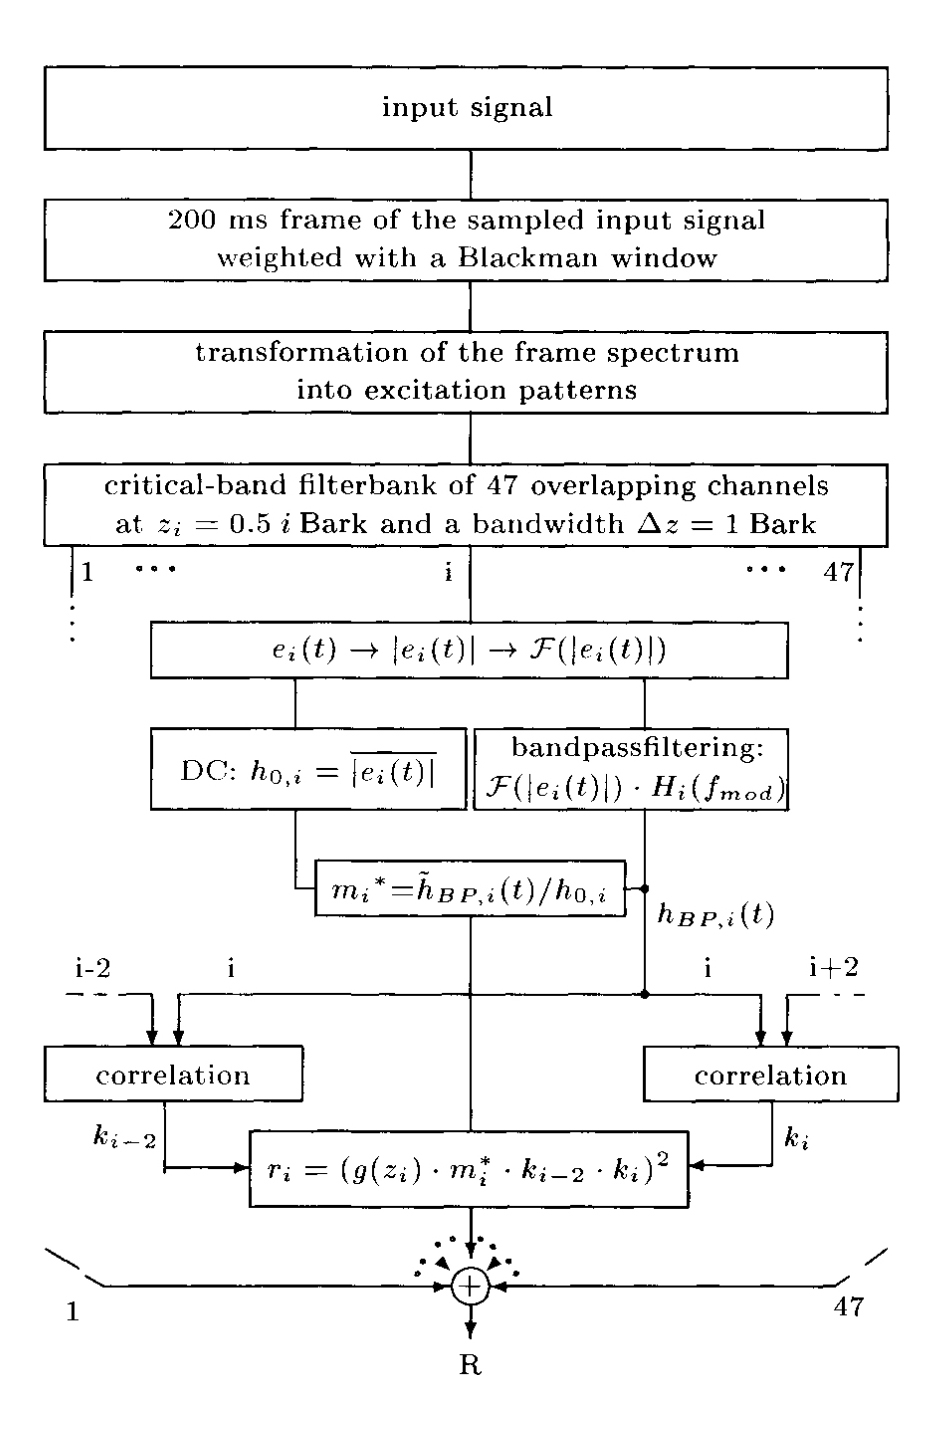
\includegraphics[height=10cm]{roughness_model}
  \caption{Structure of roughness model, as presented in
    \cite[pp.~116]{daniel1997psychoacoustical}}
  \label{fig:roughness_model}
\end{figure}

\subsection{Peripheral Stage}

First, the input signal is divided into frames, which in the original roughness
model have a 200 ms duration. For the fluctuations strength case this must be
increased, in order to achieve higher frequency detail resolution and be able
to process stimuli with frequency components with little separation among them
(e.g., $f_m = 4$ Hz). This can be achieves manipulating two variables, namely
the sampling frequency and the number of samples. For this study it has been
decided to keep the sampling frequency at 44.1 kHz, the most common frequency
used in audio recordings. The number of samples is chosen such that it contains
at least three periods of the slowest frequency component, following the
criteria presented by~\cite[pp.~97]{Boersma1993}. The slowest stimulus has a
modulation frequency of 0.25 Hz, thus three periods would constitute a 12 s
frame duration. This results in a number of samples of 1048576 ($2^{20}$) and a
duration of 23.77 s, using the closest value that is a power of 2.

After the frame separation, a Blackman window is applied to the frame to reduce
spectral leakage. Following this, the outer and middle ear transmission effects
are taken into account by transforming the frame into the frequency domain, and
multiplying its components by the parameter $a_0$, shown in \cref{fig:a0}.

\begin{figure}[!ht]
  \centering
  \includegraphics[height=8cm]{a0}
  \caption{Outer and middle ear transmission effects parameter $a_0$}
  \label{fig:a0}
\end{figure}

After this, the input frame spectrum is transformed into excitation patterns
using \citeauthor{Terhardt1979}'s approach \cite{Terhardt1979}. This method is a
non-linear one, where the lower and upper slopes of the excitation patterns
differ. The lower slopes are independent of the stimulus center frequency, and
are defined by:
\begin{equation}
  S_1 = -27 \quad \frac{\text{dB}}{\text{Bark}}
  \label{eq:lower_slopes}
\end{equation}

The upper slopes depends on the center frequency of the stimulus, and are
defined by the following equation:
\begin{equation}
  S_2 = [-24-\frac{0.23 \text{ kHz}}{f}+\frac{0.2 \text{ L}}{\text{dB}}]
  \quad
  \frac{\text{dB}}{\text{Bark}}
\end{equation}

Finally, the excitation patterns are processed using a critical-band filter with
47 channel, each on them separated by 0.5 Bark and having a bandwidth of 1 Bark.

\subsection{Modulation Depth Extraction Stage}

This stage's objective is to come up with an approximation of the modulation
depth present in the incoming frame on a channel basis. For each channel signal
$e_{i}(t)$ its absolute value is obtained and its mean is then calculated with
\cref{eq:h0i}.

\begin{equation}
  h_{0,i} = \overline{|e_{i}(t)|}
  \label{eq:h0i}
\end{equation}

The mean is then subtracted to each signal and the resulting signal is filtered
using a bandpass filter $H[f_{mod}]$, shown in \cref{eq:hBPi}.

\begin{equation}
  h_{BP,i}(t) = ([|e_{i}(t)| - h_{0,i}] * H[f_{mod}])(t)
  \label{eq:hBPi}
\end{equation}

Finally, the modulation depth per channel is obtained by the ratio of the
\gls{RMS} value of the bandpass filtered signal and its mean, shown in
\cref{eq:mi*}.

\begin{equation}
  {m_i}^* = \tilde{h}_{BP,i}(t)/h_{0,i}
  \label{eq:mi*}
\end{equation}

Two changes are introduced in this stage to adapt the model behavior to the
fluctuation strength scenario. First, an unique filter is used for all the 47
channels, whereas in the roughness model a different filter is used for each
channel, to take into account possible effect of the center frequency on the
modulation frequency dependency. Second, since the bandpass filter response
defines the modulation depth dependence, by adjusting it a better fit for the
fluctuation strength case can be achieved

On an implementation note with regard to the bandpass filter, the filtering is
done using a Butterworth \gls{IIR} filter. Its parameters are detailed in
\cref{tab:bandpass_filter}.

\begin{table}[!ht]
  \centering
  \begin{tabu}{l l}
    \toprule
    \rowfont\bfseries
    Parameter & Value \\
    \midrule
    Stopband Frequency 1 & 0.5 [Hz] \\
    \midrule
    Passband Frequency 1 & 2 [Hz] \\
    \midrule
    Passband Frequency 2 & 8 [Hz] \\
    \midrule
    Stopband Frequency 2 & 32 [Hz] \\
    \midrule
    Stopband Attenuation 1 & 100 [dB] \\
    \midrule
    Passband Ripple & 3 [dB] \\
    \midrule
    Stopband Attenuation 2 & 100 [dB] \\
    \bottomrule
  \end{tabu}
  \caption{Bandpass filter characteristics}
  \label{tab:bandpass_filter}
\end{table}

\subsection{Specific Roughness Stage}

The last stage of the model deals with the specific roughness calculation. The
model is based on the dependence of roughness on modulation depth, portrayed
by \cref{eq:roughness_modulation_depth}.

\begin{equation}
  R \sim m^p
  \label{eq:roughness_modulation_depth}
\end{equation}

For each channel, a specific value of roughness is obtained by using the
\cref{eq:ri}.

\begin{equation}
  r_i = [g(z_i) \cdot {m_i}^* \cdot k_{i-2} \cdot k_i]^2
  \label{eq:ri}
\end{equation}

The parameter $g(z_i)$ corresponds to a weight associated to each channel, and
it models the dependence of roughness on the center frequency of the stimulus.
Additionally, cross correlations between the prior and the posterior channel
are included ($k_{i-2}, k_i$) to account for phase shifts of the channels
signals. The total roughness is then obtained by summing all the specific
values for each channel, shown in \cref{eq:total_roughness}, where cal is a
calibration constant.

\begin{equation}
  R = \text{cal} \cdot \displaystyle\sum_{i=1}^{47} r_i
  \label{eq:total_roughness}
\end{equation}

In order to accommodate for the fluctuation strength scenario, a different
equation for the specific fluctuation values was proposed, that provided more
flexibility to adapt the model response to the obtained data. First, the three
factors used in the specific value calculation where assigned a separate power
coefficient to them, shown in \cref{eq:fi}. In this way, each contribution of
these components can be weighted and adjusted individually.

\begin{equation}
  f_i = [g(z_i)]^{p_g} \cdot [{m_i}^*]^{p_m} \cdot [k_{i-2} \cdot k_i]^{p_k}
  \label{eq:fi}
\end{equation}

After the adjustments, the parameter $g(z_i)$ was removed, since the data
gathered did not show a dependence on the center frequency. Furthermore, to
avoid imaginary values when using power coefficients lesser than 1, the absolute
value of the product of the cross correlations coefficients was used. Although
this negates the substraction of specific fluctuation due to a negative
coefficient, it yields better fitting results. The final form of the specific
fluctuation strength equation is shown in \cref{eq:fi_final}.

\begin{equation}
  f_i = [{m_i}^{*\prime}]^{0.25} \cdot |k_{i-2} \cdot k_i|^{0.375}
  \label{eq:fi_final}
\end{equation}

where

\begin{align}
  {m_i}^{*\prime} &= H({m_i}^{*\prime\prime}) \cdot {m_i}^{*\prime\prime}
  \label{eq:md_transformation_1} \\
  {m_i}^{*\prime\prime} &= {m_i}^* - 0.1
  \label{eq:md_transformation_2}
\end{align}

being $H$ the Heaviside step function.

The total fluctuation strength is then obtained using
\cref{eq:total_fluctuation}.

\begin{equation}
  F = 0.15 \cdot \displaystyle\sum_{i=1}^{47} f_i
  \label{eq:total_fluctuation}
\end{equation}

\section{Procedure}

The parameters were adjusted using the following order:
\begin{inparaenum}[(1)]
  \item $p_m$,
  \item $p_k$,
  \item cal,
  \item $H(f_{mod})$.
\end{inparaenum}
The order are order such that the first parameter has the most spread effect
of change among all the response curves. Furthermore, the goodness of fit of the
model was judged both from a quantitative and a qualitative point of view, by
comparing the model and experiment curves, and by using the sum of the square of
the difference between these ($\sum r_i^2$).

Parameter $p_m$ modifies directly the effect of modulation depth on fluctuation
strength. Since the model is based on this relation, it affects all the model
response curves, and as so it was the first parameter to adapt. The power
coefficient had to be drastically reduced from the value of 2, present in the
original roughness model, to a value of 0.25, to account for the fast increment
of fluctuation values as the modulation depth increased present in the dataset.
Furthermore, a transformation was needed
(\cref{eq:md_transformation_1,eq:md_transformation_2}) to correct for the higher
values caused by the power coefficient change for lower values of
modulation depth.

Parameter $p_k$ has a predominant effect on \gls{FM} tones, specially on the
dependency of frequency deviation, center frequency and modulation frequency.
After adjusting this parameter the calibration constant cal was adjusted to
attain a value of 1 vacil for the reference tone, present in the AM-SPL curve.

Finally, the bandpass filter was adjusted, this having a effect mostly on the
modulation frequency dependency for both types of tones.

\section{Results}

The following are the results of the model compared with the obtained
experimental data.

\modelresultsfigure{am-fm}{modulation frequency}{AM}
\modelresultsfigure{am-fc}{center frequency}{AM}
\modelresultsfigure{am-spl}{sound pressure level}{AM}
\modelresultsfigure{am-md}{modulation depth}{AM}
\modelresultsfigure{fm-fm}{modulation frequency}{FM}
\modelresultsfigure{fm-fc}{center frequency}{FM}
\modelresultsfigure{fm-spl}{sound pressure level}{FM}
\modelresultsfigure{fm-df}{frequency deviation}{FM}

The model adapts better to the AM tones than to the FM tones, reporting lower
values of $\sum r_i^2$ in the former case than in the latter. However, from a
qualitative point of view, the responses obtained for FM tones tend to follow
the ones present in the experimental data, albeit with systematic level
differences, especially in the case of center frequency and frequency deviation.

\end{modelchapter}

\end{document}
